\subsection{Microelectronics Materials and Devices}
\subsubsection{Crystal Structure}
\begin{enumerate}
    \item Type of solids: \\
    Solids are ordered according to 3 types: amorphous, polycrystalline, and single crystal.
    \begin{figure}[h]
        \centering
        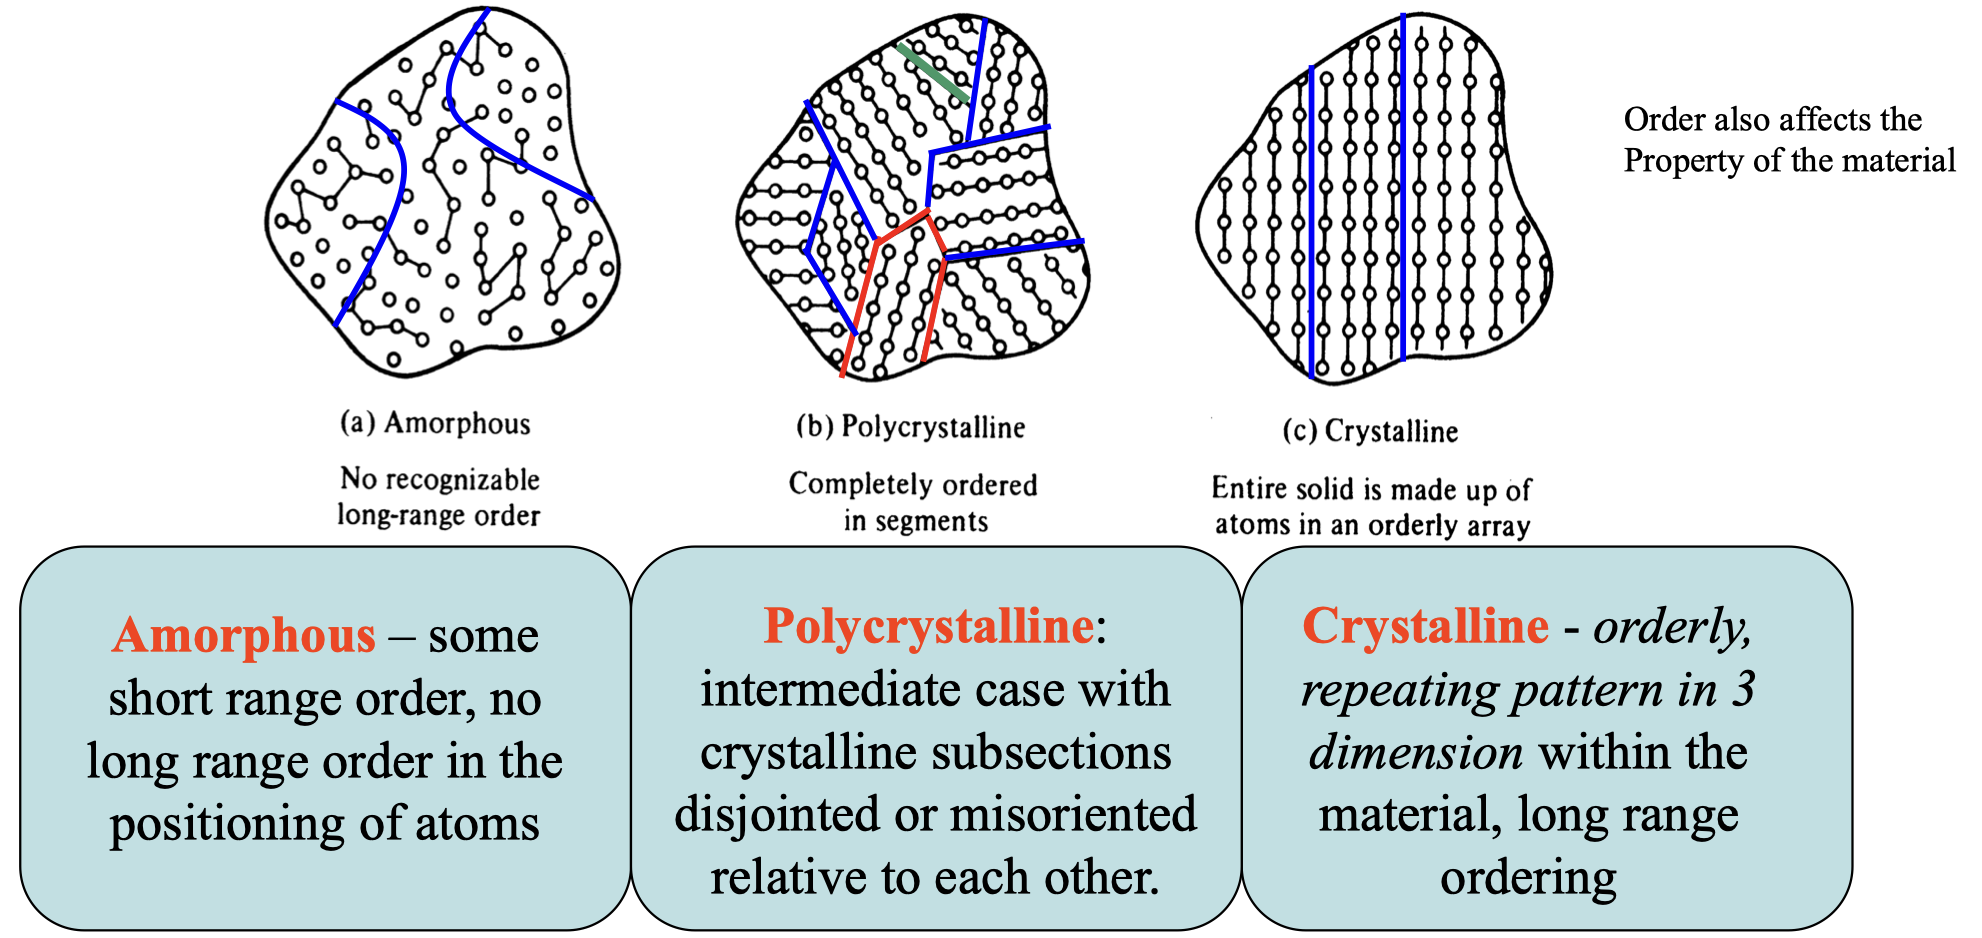
\includegraphics[width=0.75\linewidth]{image/crstal.png}
    \end{figure}
    \item How to describe a crystal structure\\
    Crystal Structure = Lattice Point + Basis \\
    Basis = single atom OR group of atoms attached to each lattice point \\
    \begin{figure}[h]
        \centering
        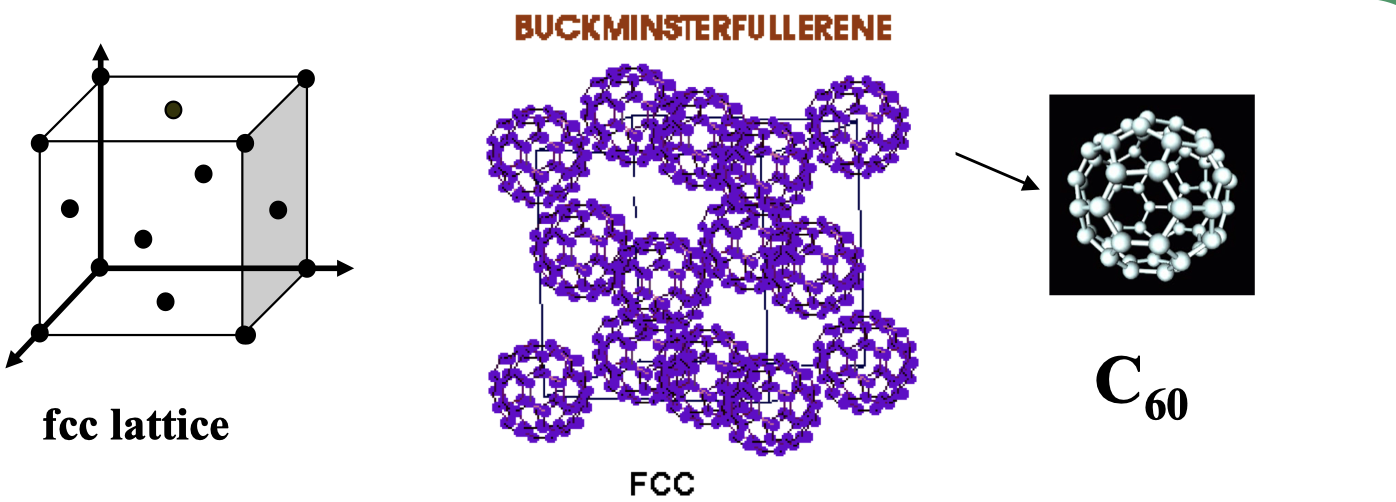
\includegraphics[width=0.8\linewidth]{image/latticestructure.png}
    \end{figure}
    \item Unit Cell \\
    Unit Cell = small portion of any given crystal that can be used to reproduce the crystal. \\
    Lattice angles: the inter-axial angles $\alpha$, $\beta$ and $\gamma$. \\
    Lattice constants: all of the parameters of the unit cell. \\
    Volume: $\displaystyle V = |\Vec{a}\cdot\Vec{b}\times\Vec{c}|$
    \begin{figure}[h]
        \centering
        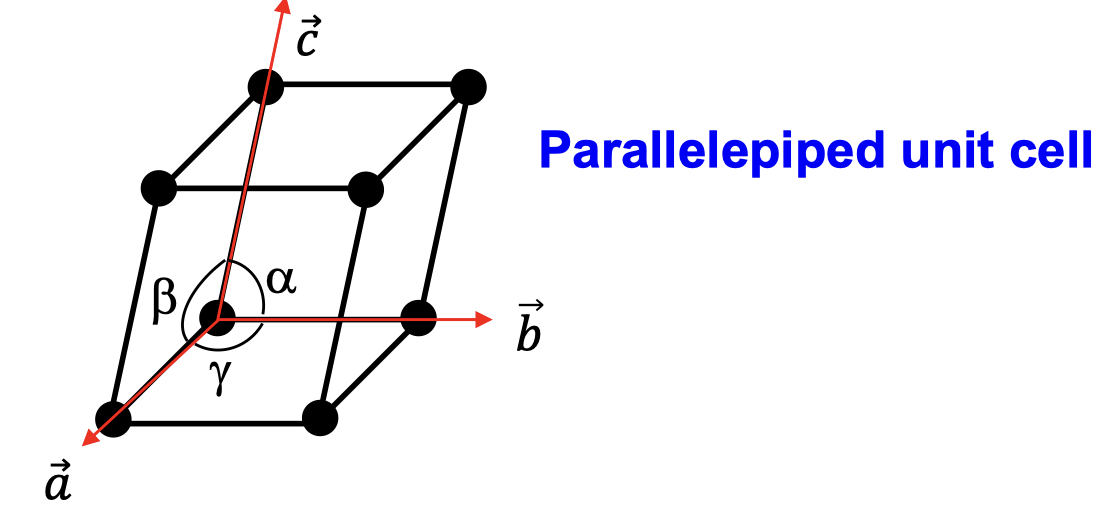
\includegraphics[width=0.75\linewidth]{image/unicell.png}
    \end{figure}
    \item 3D Bravais Lattice Types
    There are only 14 \textbf{unique} Bravais Lattices (unit cells) to fill space with a periodic arrangement of points. \\
    The ones we are interested are: bcc, fcc and hcp.
    \begin{figure}[h]
        \centering
        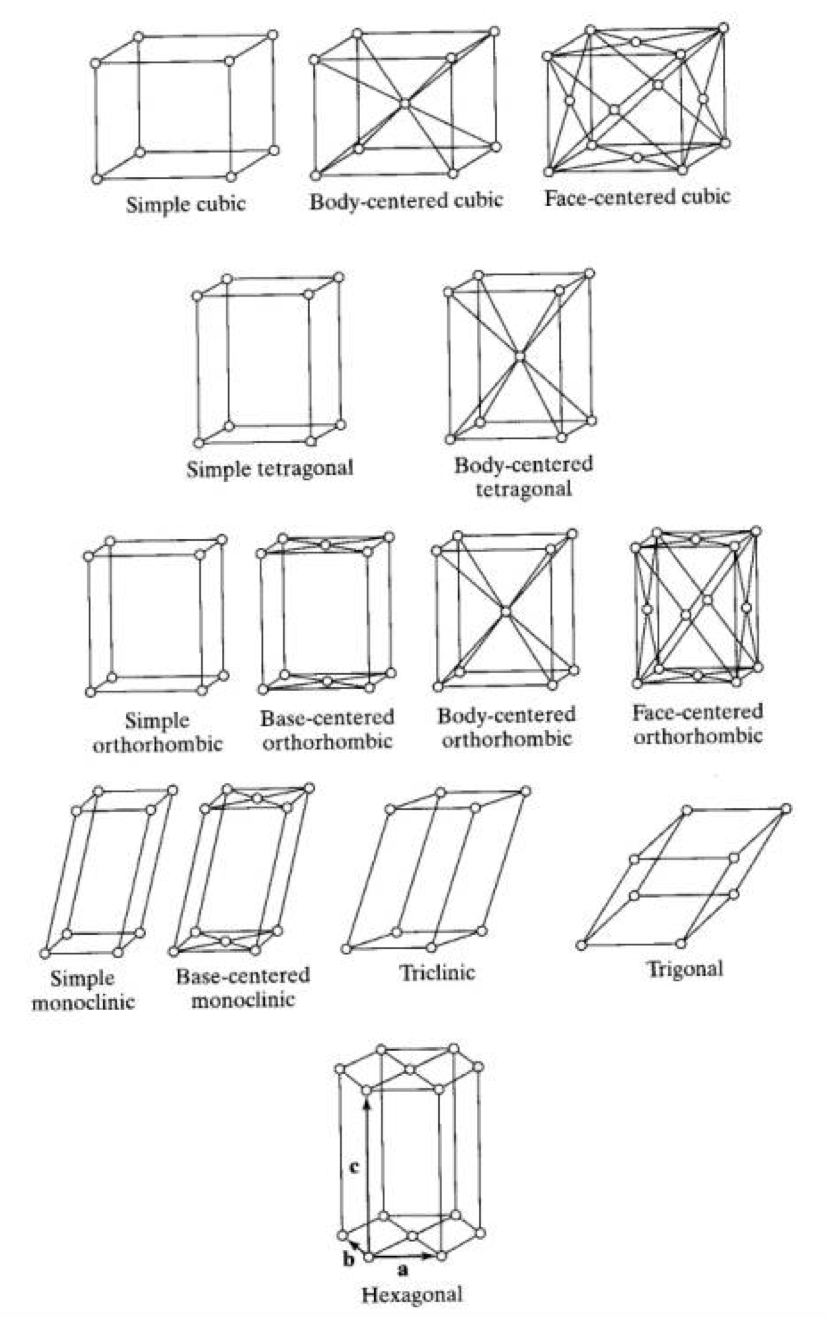
\includegraphics[width=0.5\linewidth]{image/14cellls.png}
    \end{figure}
    \item Cubic Lattices\\
    \begin{figure}[h]
        \centering
        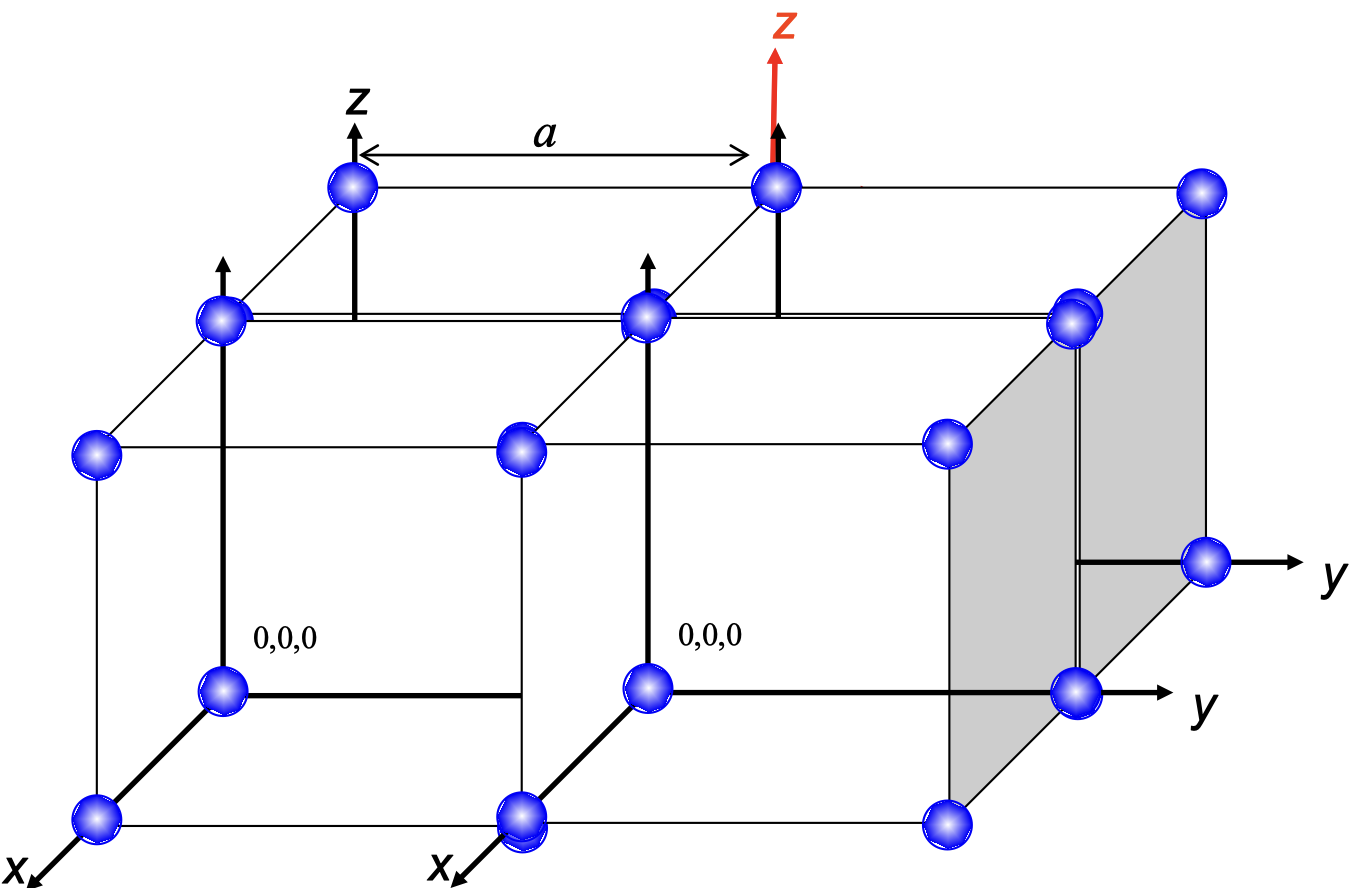
\includegraphics[width=0.75\linewidth]{image/cubiclattic.png}
    \end{figure}
    Cubic lattices can be specified by a single lattice constant \textcolor{red}{a}. \\
    Note: Since each atom is shared by 8 unit cells, only 1/8 of each corner atom is inside each unit cell. \\
    Example of SC Metals : \ce{Po}
    \item Body-centred Cubic (Bcc) Structure
    \begin{figure}[h]
        \centering
        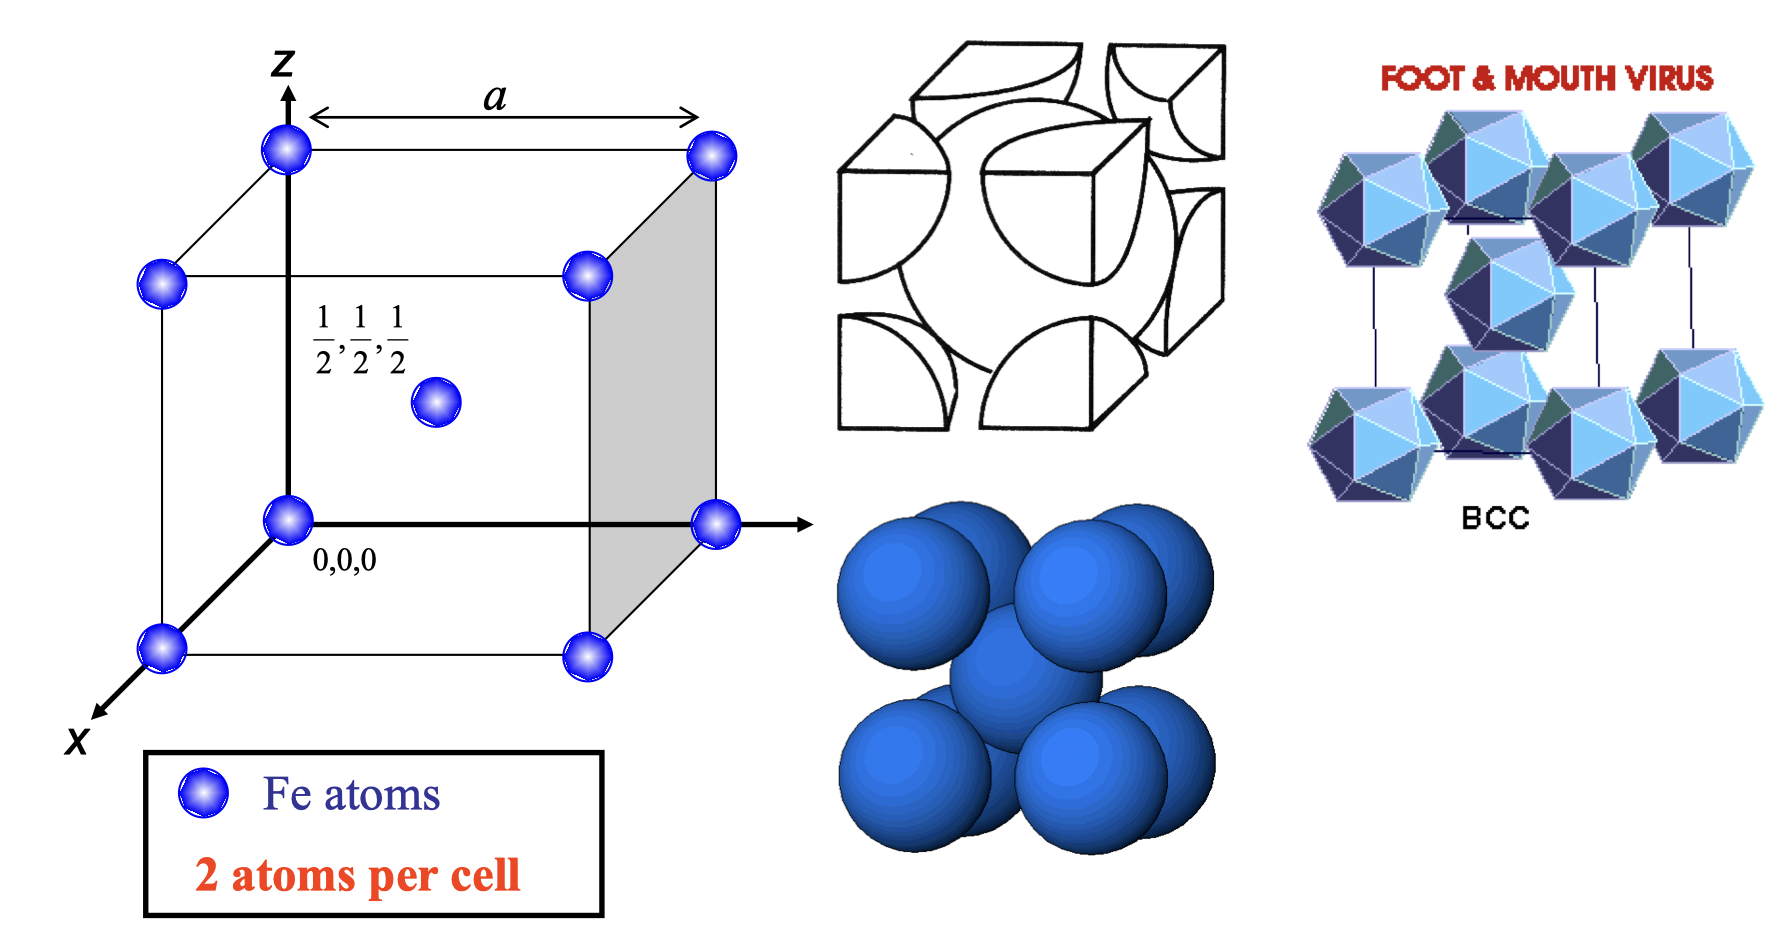
\includegraphics[width=0.75\linewidth]{image/bcc.png}
    \end{figure} \\
    Example of Bcc Metals: \ce{Fe}, \ce{W}, \ce{Mo}, \ce{Nb}, \ce{Ta}, \ce{V}, \ce{Cr}
    \newpage
    \item Face-centered Cubic (Fcc) Structure 
    \begin{figure}[h]
        \centering
        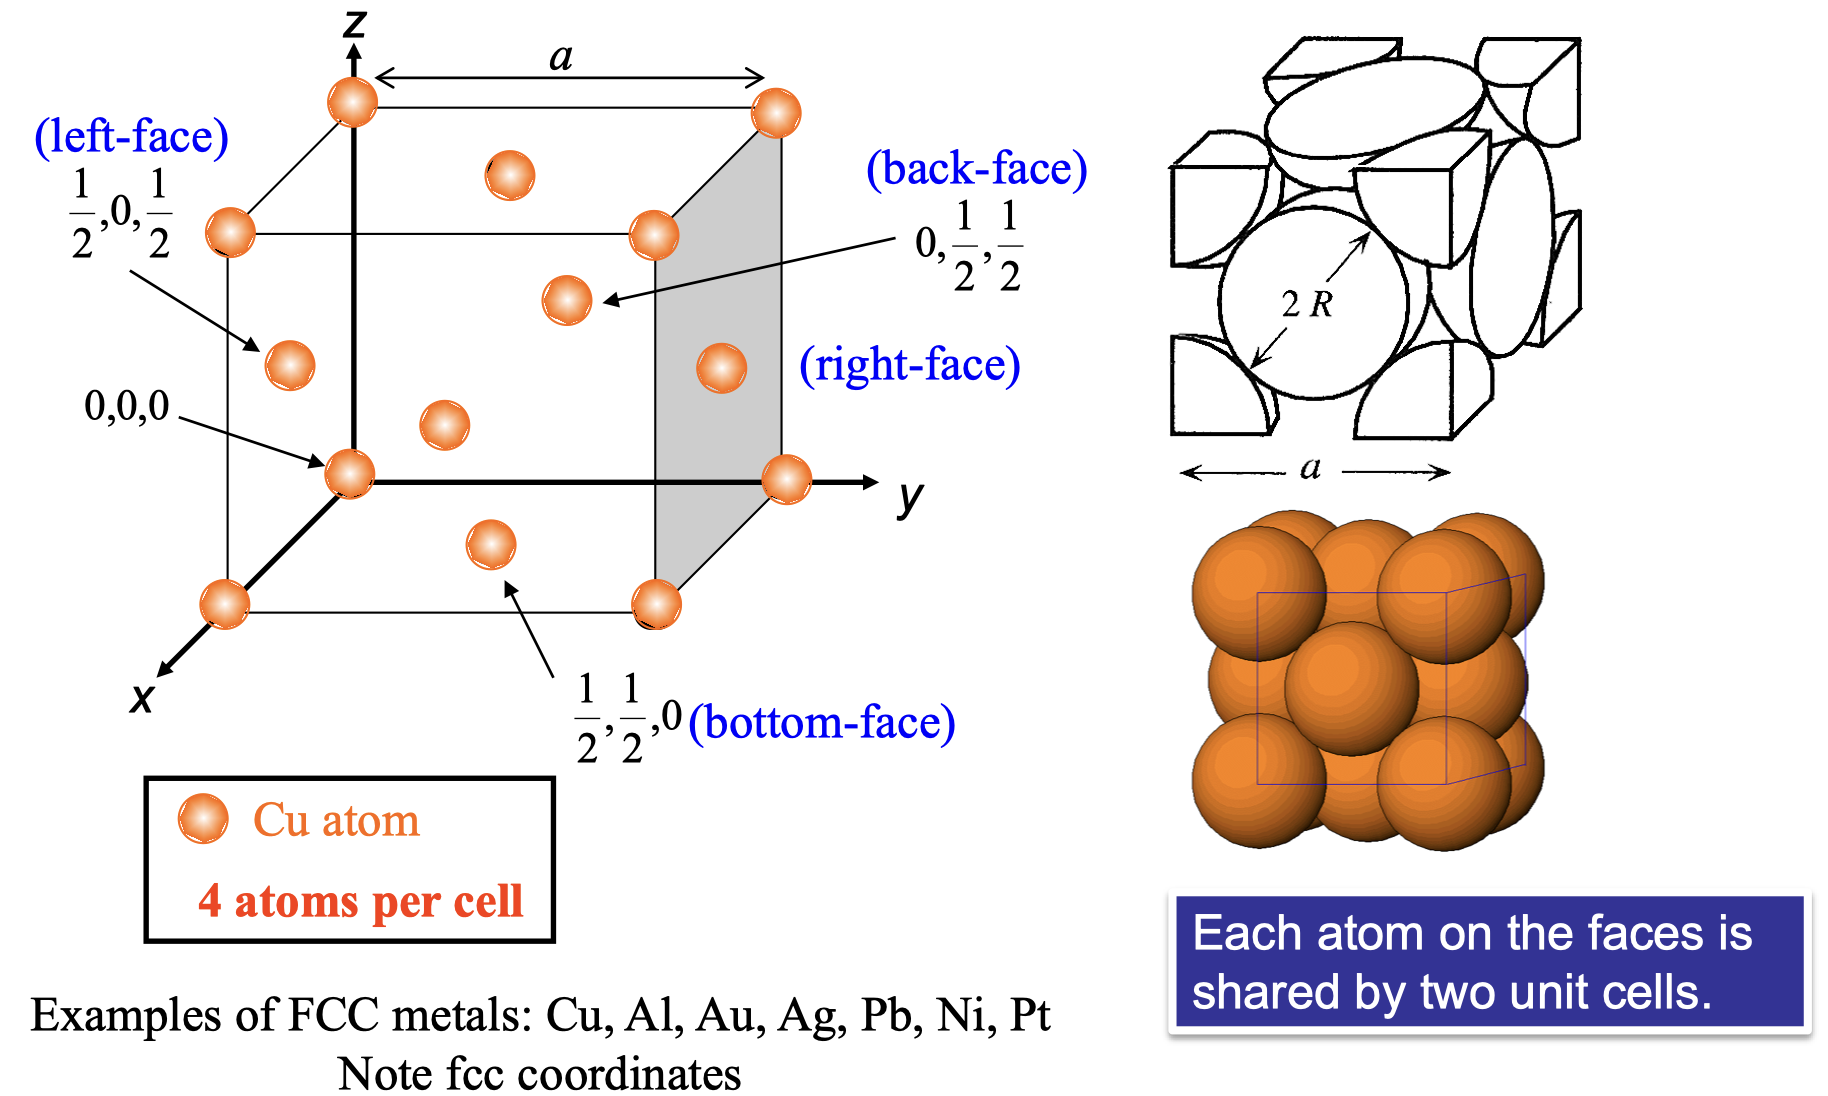
\includegraphics[width=0.75\linewidth]{image/fcc.png}
    \end{figure}
    \item Fcc Derivatives (Diamond Structure) 
    \begin{figure}[h]
        \centering
        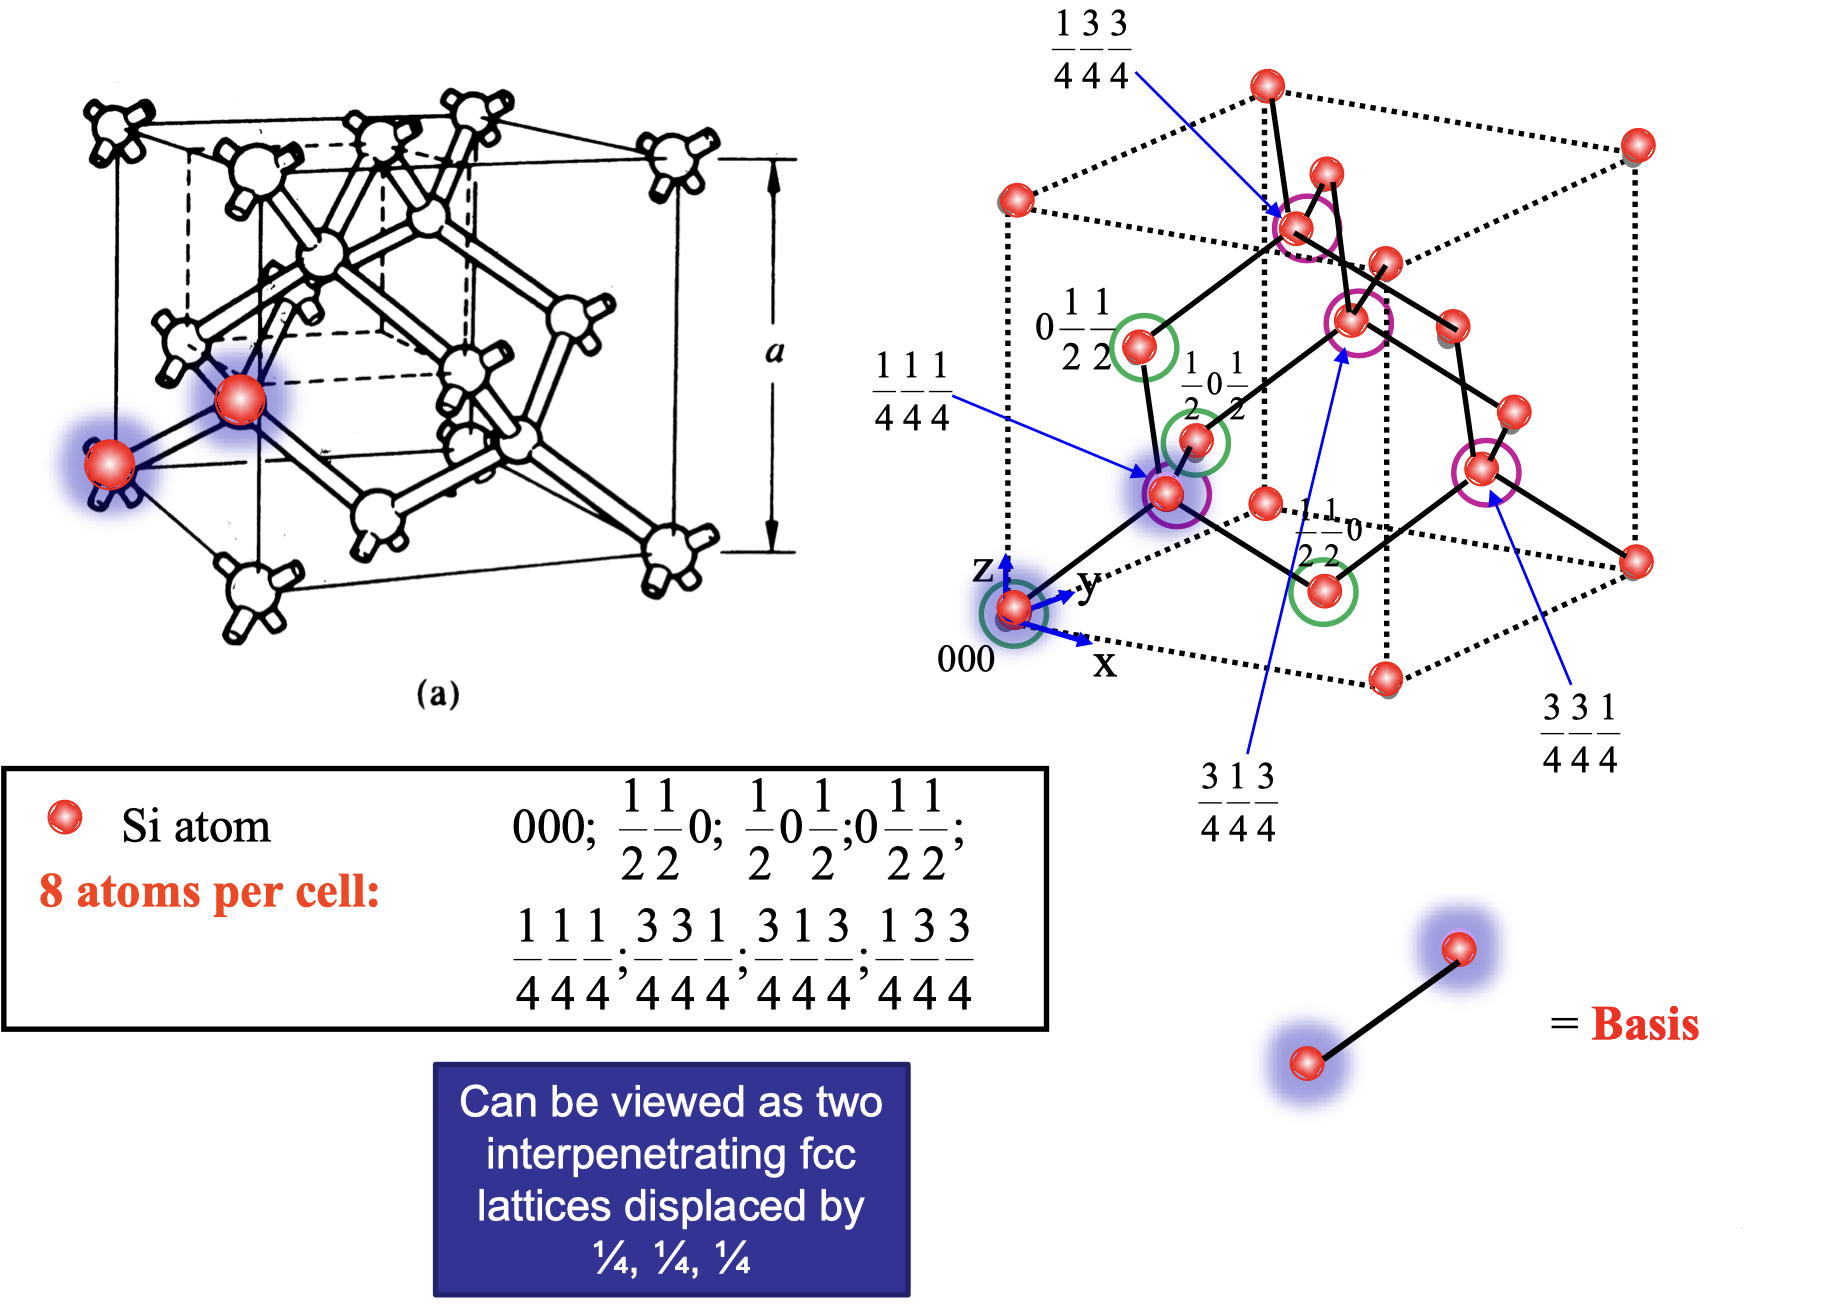
\includegraphics[width=0.75\linewidth]{image/diamondsturc.png}
    \end{figure} 
    \newpage
    \item Fcc Derivatives (Zinc-Blende Structure) 
    \begin{figure}[h]
        \centering
        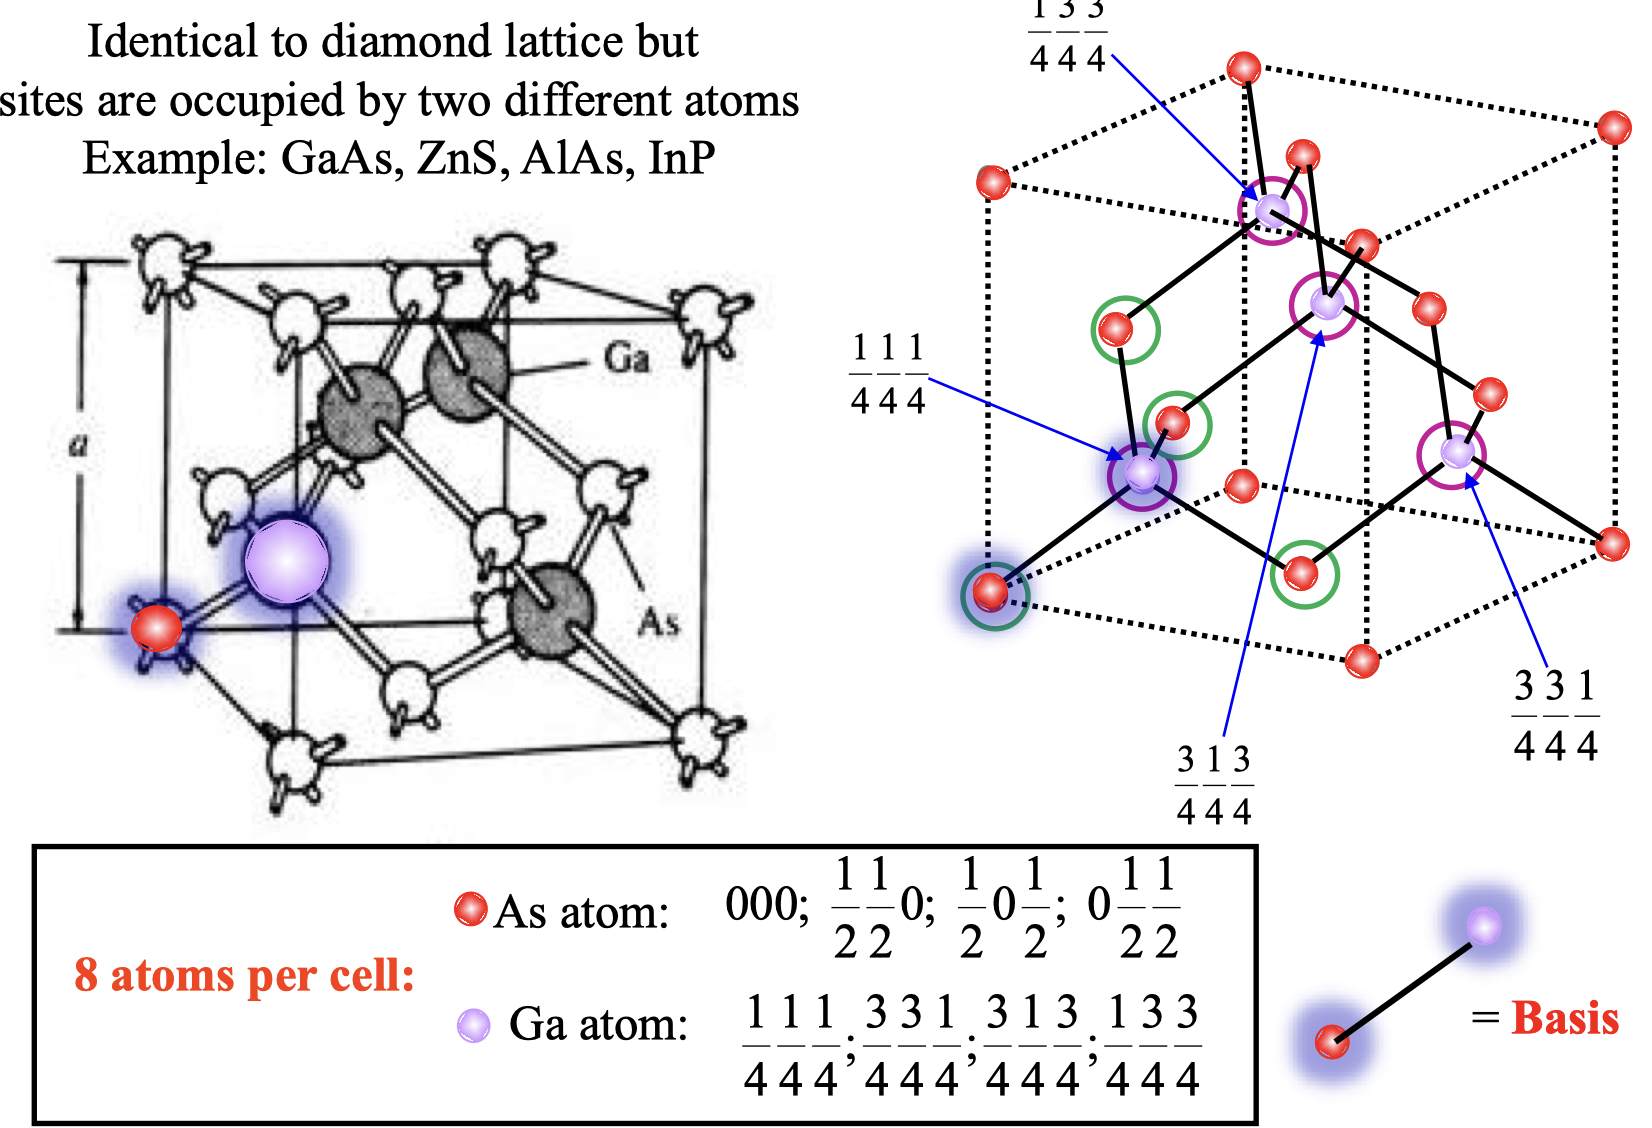
\includegraphics[width=0.75\linewidth]{image/zincblende.png}
    \end{figure}
    \item Sodium Chloride (Rocksalt) structure
    \begin{figure}[h]
        \centering
        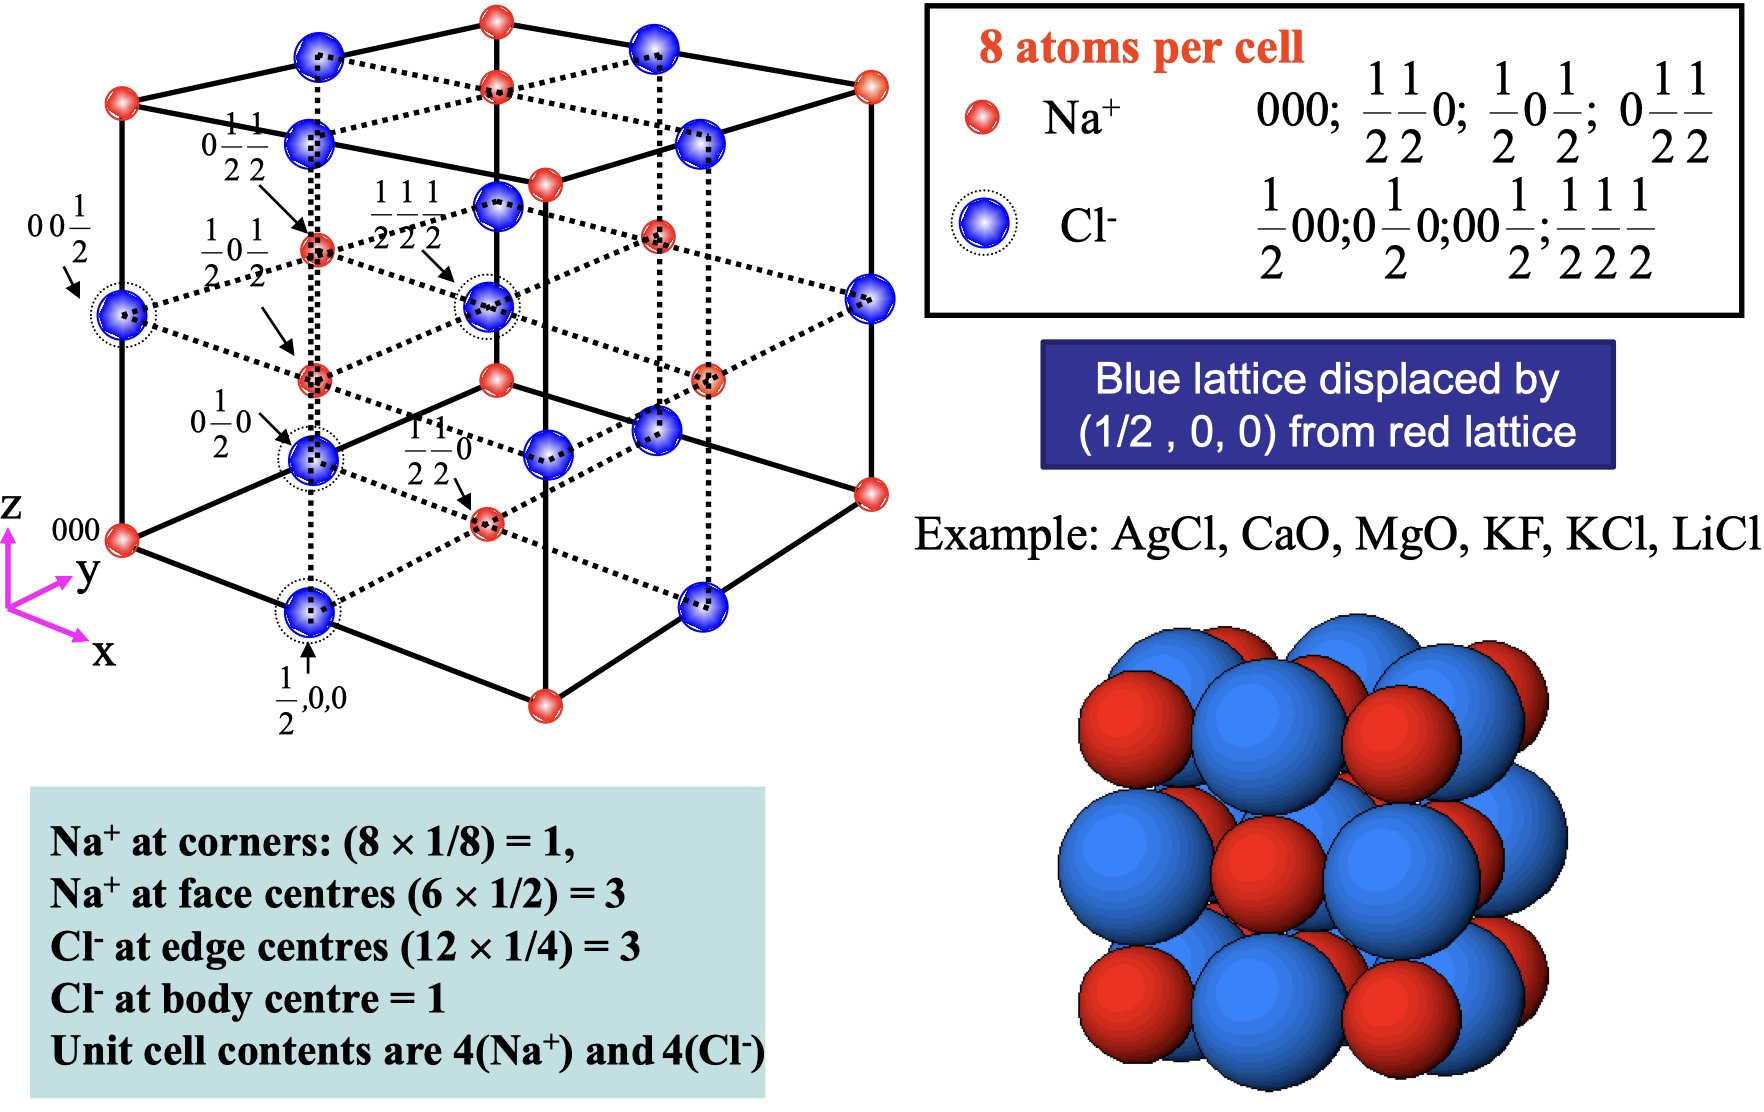
\includegraphics[width=0.75\linewidth]{image/rockcet.png}
    \end{figure}
    \newpage
    \item Hexagon lattice \\
    In 2D, close packed layers is the most efficient way of packing equal sized spheres. They can be stacked to closely packed to give 3D structure.
    \begin{figure}[h]
        \centering
        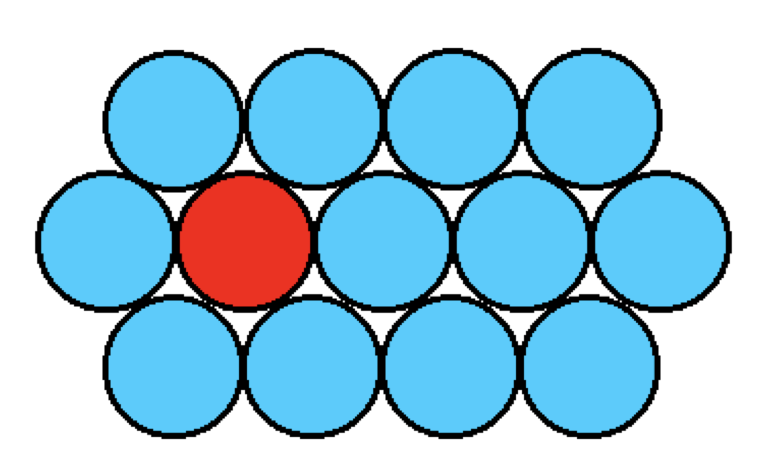
\includegraphics[width=0.5\linewidth]{image/2dgraph.png}
    \end{figure} \\
    It can have A position sequence $\ldots ABABABAB\ldots$ and this is  Hexagonal close packing (hcp). \\ 
    It can also position sequence $\ldots ABCABCABCABC\ldots$ and this is  Cubic close packing (ccp). \\
    The difference between hcp and ccp
    \begin{figure}[h]
        \centering
        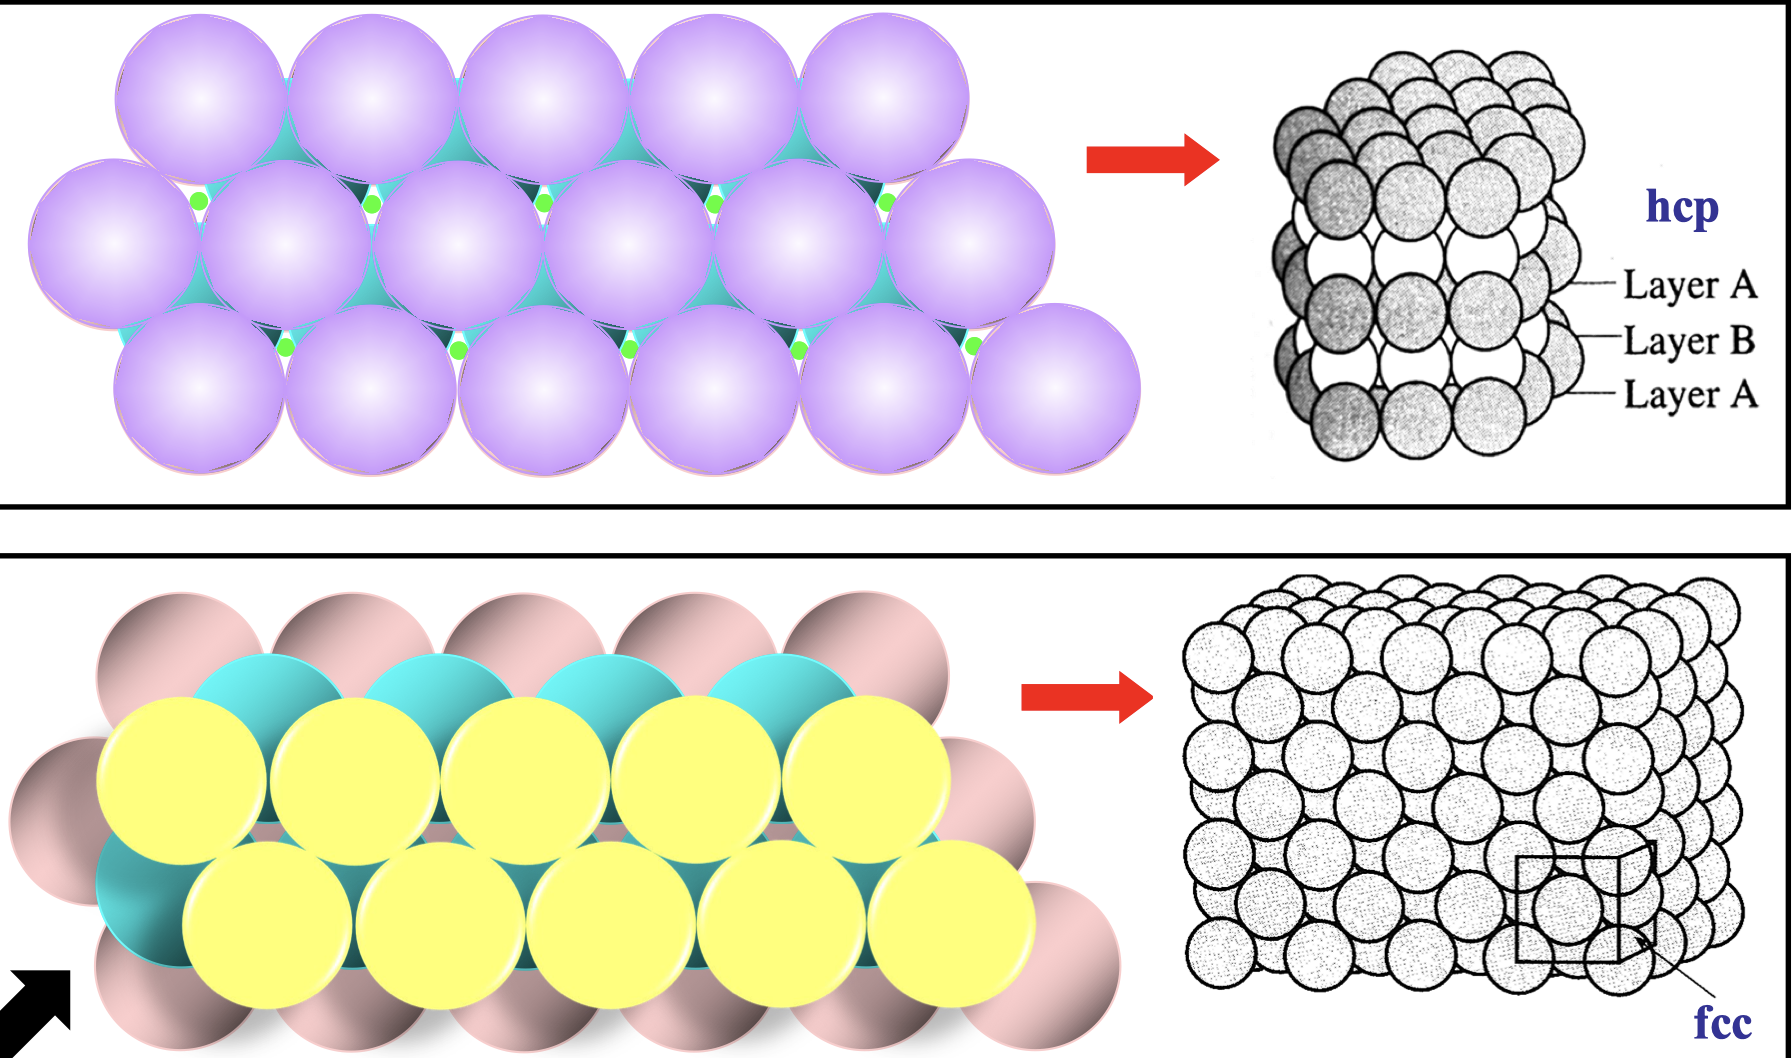
\includegraphics[width=0.75\linewidth]{image/hcpccp.png}
    \end{figure}
    \item Hexagonal System (Number of atoms)
    \begin{figure}[h]
        \centering
        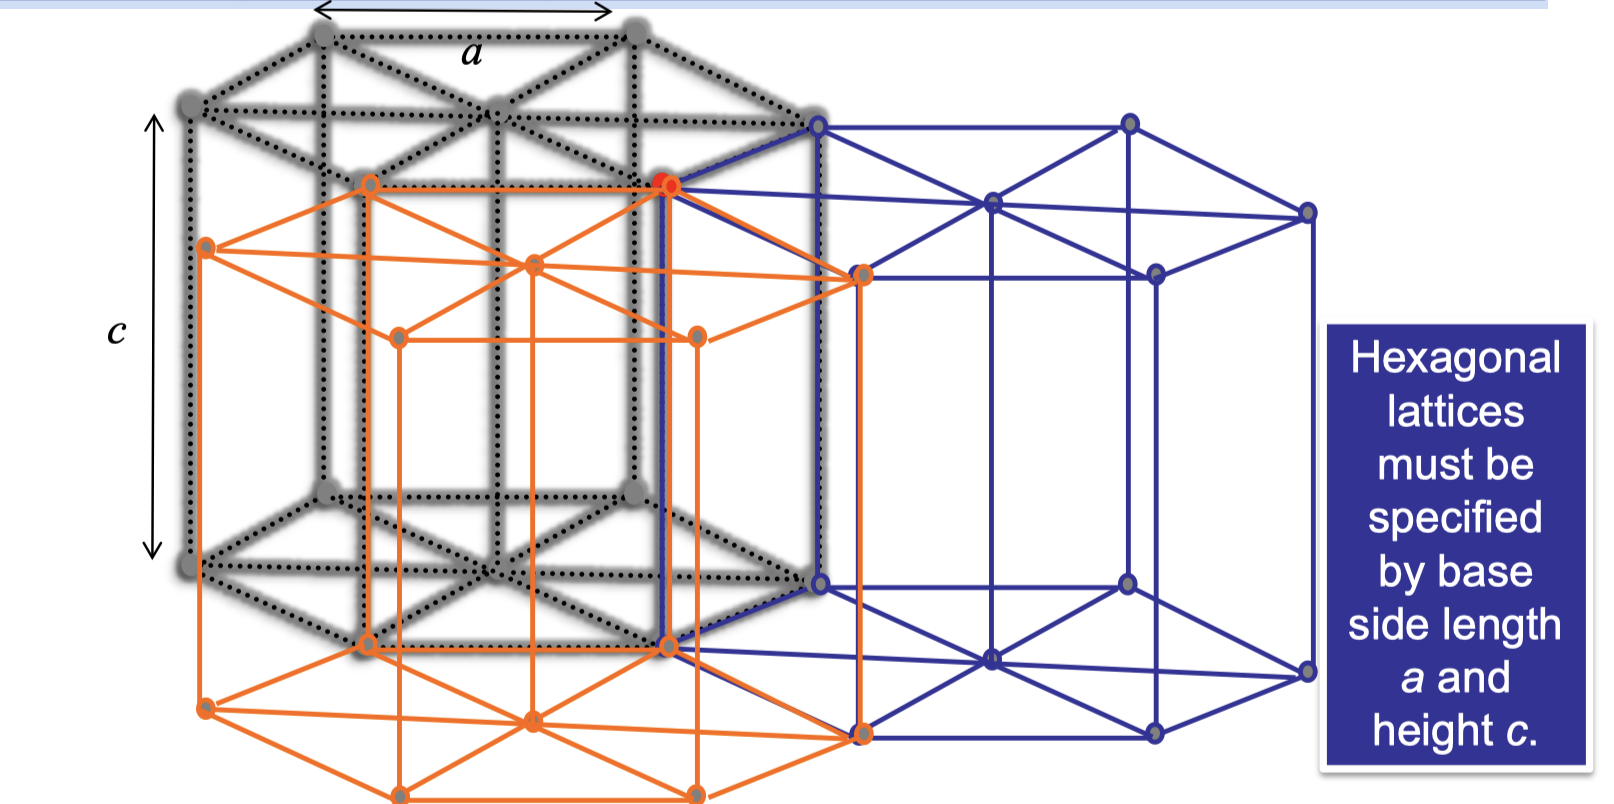
\includegraphics[width=0.5\linewidth]{image/hcpno.png}
    \end{figure} \\
    Number of atoms per unit cell = 3.\\
    Each corner atom shared with 6 neighbour cells. Total 12 neighbour gives 2 atoms. $\frac{1}{6} \times 12 = 6$\\
    The centered atom at the top and bottom of the cell shared half with neighboring cell. $\frac{1}{2} \times 2 = 1$ \\
    In total: $2+1 = 3$.
    \item Atomic Packing Factor \\
    Maximum fraction of the volume in a unit cell occupied by the atoms.\\
    Assume that the atoms are closely packed and that they can be treated as hard spheres. This fraction is called atomic packing factor (APF) or packing density.
    \[APF = \frac{\text{Number of atoms per cell $\times$ volume of one atom}}{\text{volume of unit cell}}\]
    \vspace{1cm}
    \begin{minipage}{0.5\textwidth}
        Number of atoms: 4 \\
        Volume of each atoms: $\displaystyle \frac{4}{3}\pi R^3$ \\
        Unit cell Volume : $\displaystyle a^3 = (2\sqrt{2}R)^3$ \\
        $\displaystyle APF = \frac{\frac{4}{3} \pi R^3}{(2\sqrt{2}R)^3} = 0.74$
    \end{minipage}
    \begin{minipage}{0.5\textwidth}
        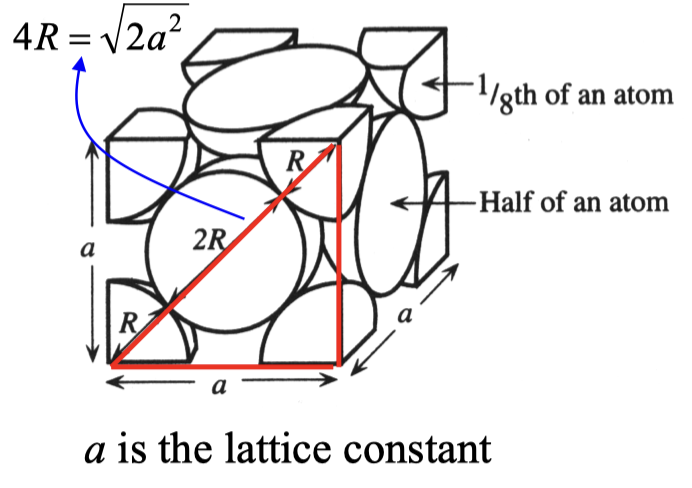
\includegraphics[width=0.75\linewidth]{image/atomcellvol.png}
    \end{minipage}
    \item Atomic Packing factor for different structures
    \begin{center}
    \begin{tabular}{|l|c|c|c|c|}
    \hline
        \textbf{Structure} & \textbf{Radius} & \textbf{Atom/unit cell} & \textbf{APF} & \textbf{Coordination no.}\\ \hline
        Simple cubic       & $\frac{a}{2}$   & 1                       & $\frac{\pi}{6} = 52\%$ & 6\\ \hline
        BCC                & $\frac{\sqrt{3}a}{4}$ & 2                 & $\frac{\pi\sqrt{3}}{8} = 68\%$ & 8\\ \hline
        FCC                & $\frac{\sqrt{2}a}{4}$ & 4                 & $\frac{\pi\sqrt{2}}{6} = 74\%$ & 12\\ \hline
        Diamond            & $\frac{\sqrt{3}a}{8}$ & 8                 & $\frac{\pi\sqrt{3}}{16} = 34\%$ & \\ \hline
    \end{tabular}
    \end{center}
    \item Miller Indices for Crystal Planes\\
    Steps to write \textit{hkl} plane notations
    \begin{enumerate}
        \item Find the plane intercepts.
        \item Take the reciprocals.
        \item Find the smallest three integers having the same ratio.
        \item Write down the indices of the plane. E.g. (233) -- (\textit{hkl})
    \end{enumerate}
    Take note that a group of equivalent planes is denoted by braces around the indices. For example, $(100),(010),(001),(\bar{1}00),(0\bar{1}0),(00\bar{1})$ are collectively denoted as $\{100\}$.
    \item Distance between adjacent (\textit{hkl}) planes.\\
    \begin{equation}
        d_{hkl} = \frac{a}{\sqrt{h^2+k^2+l^2}}
    \end{equation}
    $d$ is the distance from a selected origion containing one plane and another parallel plane with the same indices which is closest to it.
    \item Directions in Crystal \\
    Family of directions can be represented by : $<100>$
    \item Crystal-direction vector \\
    For a cubic crystal, the angle $\theta$ between directions $[h_1k_1l_1]$ and $[h_2k_2l_2]$ is given by
    \begin{equation}
        \cos \theta = \frac{h_1h_2+k_1k_2+l_1l_2}{\sqrt{(h_1^2+k_1^2+l_1^2)(h_2^2+k_2^2+l_2^2)}}
    \end{equation}
    An typical application of Miller indices is Crystal Plane and Crystal Directions.
    \item Atomic Concentration 
    \[\text{Atomic concentration} = \frac{\text{Number of atoms}}{\text{unit volume}}\]
    \item Volume Density 
    \begin{align*}
        \rho_\nu &= \frac{\text{Mass of all atoms in the unit cell}}{\text{volume of the unit cell}} \\
        &= \text{Atomic concentration} \times \text{mass}
    \end{align*}
    \item Planar concentration 
    \[\text{Planar concentration} = \frac{\text{no. of atoms who centers are intersected by area }}{\text{area}}\]
    \newpage
    \item X-ray and diffraction grating \\
    Bragg's Law
    \begin{equation}
        2d_{hkl}\sin \theta= n\lambda
    \end{equation}
    \begin{figure}[h]
        \centering
        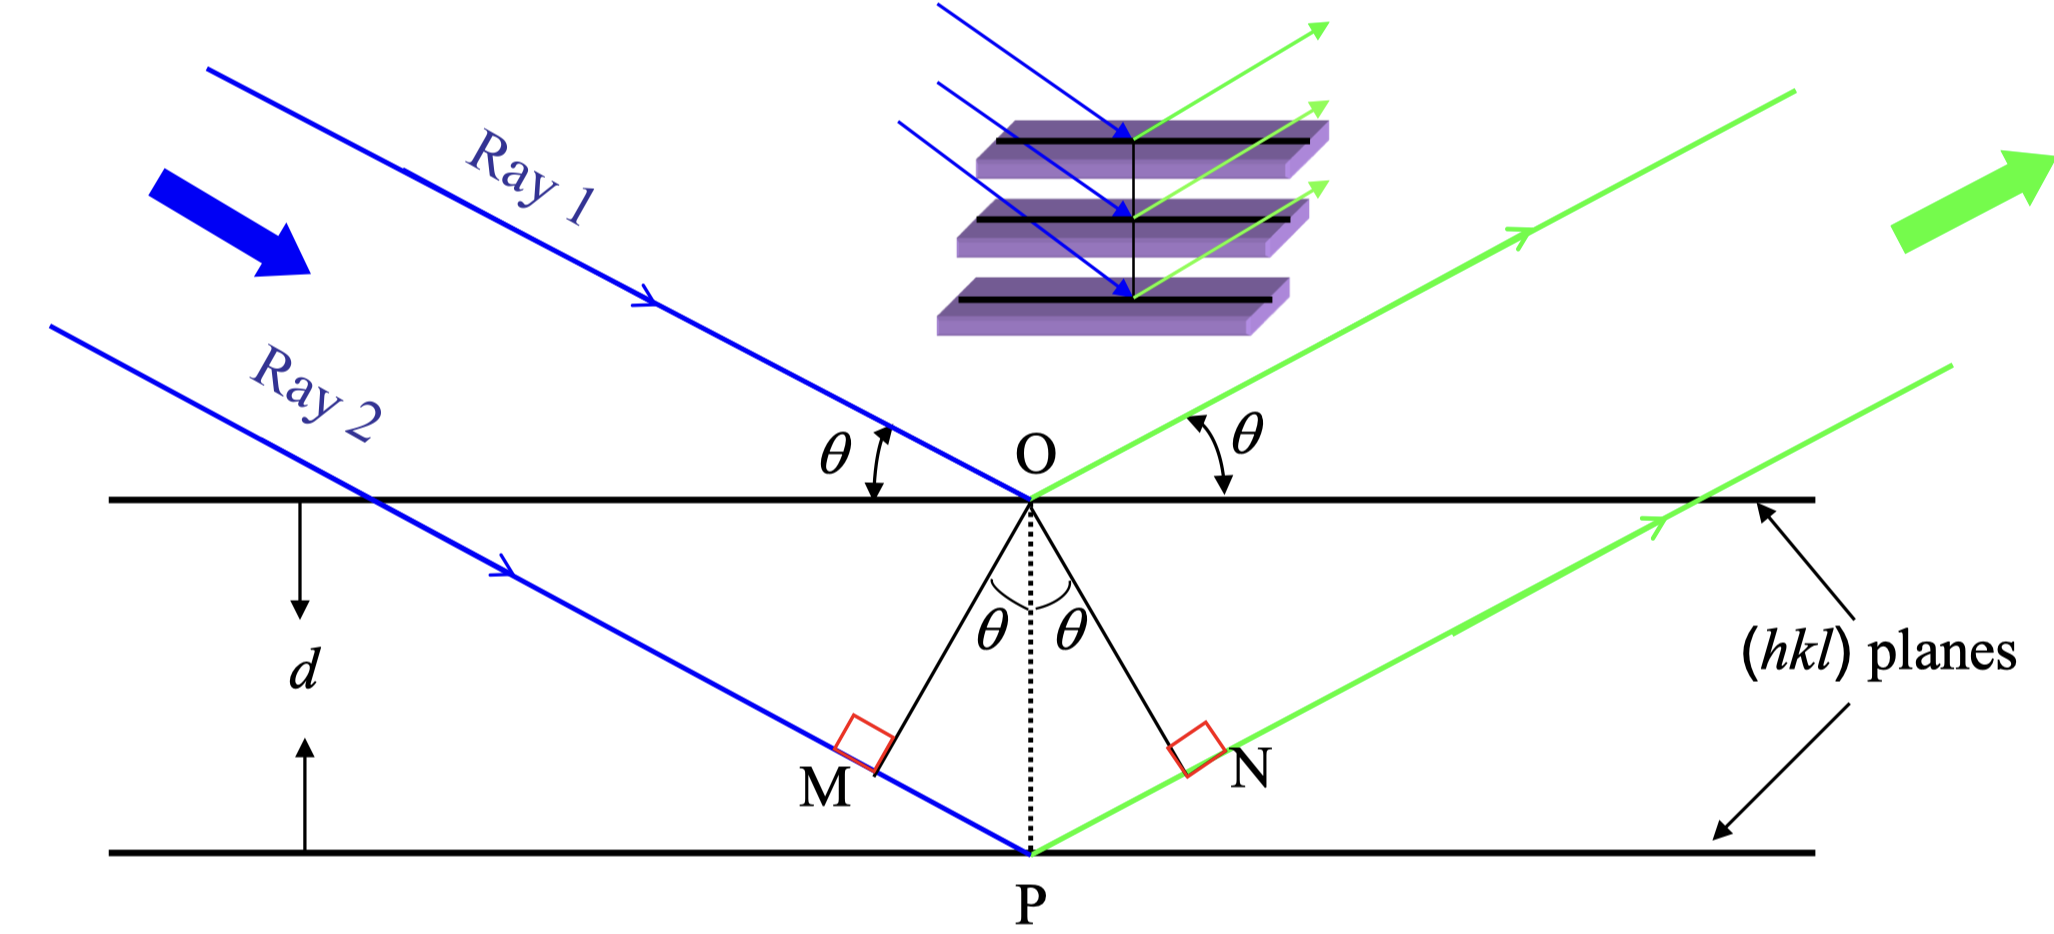
\includegraphics[width=0.75\linewidth]{image/bragglaw.png}
    \end{figure}
    For constructive interference $\displaystyle n\lambda = MP + PN$ \\
    Take note that  the higher the planar concentration (or planar density) in a crystalline material, the higher the intensity of the peak in an X-ray diffraction (XRD).
    
\end{enumerate}
\subsubsection{Band Theory}
\begin{enumerate}
    \item Bohr Atomic Model \\
    The voltage due to charge at radius $r$ is 
    \[V(r) = \frac{+e}{4\pi \varepsilon_0 r}\]
    Potential Energy is
    \[E_{PE}(r) = Q\cdot V = \frac{-e^2}{4\pi \varepsilon_0 r}\]
    Take note that $\varepsilon_0 = 8.85\times 10^{-12} F/m$ \\
    Kinetic energy of the orbiting electron is 
    \[E_{KE}(r) = \frac{e^2}{8\pi \varepsilon_0 r}\]
    Total energy is 
    \[E_{tot}(r) = E_{PE}+E_{KE} = \frac{-e^2}{8\pi \varepsilon_0 r}\]
    According to Bohr atomic model, electrons can only exist at fixed radii given by 
    \begin{equation}
        r_n = n^2 \hbar^2 \frac{4\pi \varepsilon_0}{m_0 e^2}\; :\; n = 1,2,3\ldots 
    \end{equation}
    Where $m_0 = 9.108\times 10^{-31} kg$ and $\hbar = \frac{h}{2\pi}$, $h = 6.625\times 10^{-34} J.s$
    \item Electronic Configuration \\
    \begin{figure}[h]
        \centering
        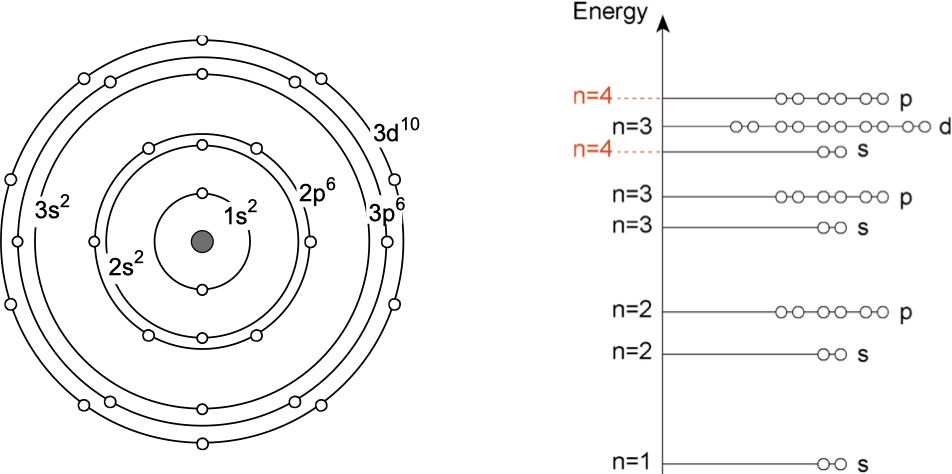
\includegraphics[width=0.75\linewidth]{image/eleconifg.png}
    \end{figure}
     \\
    \item Band Theory-Energy Levels in Atoms \\
    Split in energy level when shells overlap. \\
    The degree of split depends on the extent of the overlap. \\
    Electrons will fill up the lowest possible energy states. \\
      \\
    \begin{minipage}{0.5\textwidth}
        For a large number of atoms, a band of very closely-spaced discrete energy levels is formed from each atomic energy level. \\
        The separation between energy levels is very small. Hence the values of energy an electron can have within a band is quasi-continuous.
    \end{minipage}
    \begin{minipage}{0.4\textwidth}
        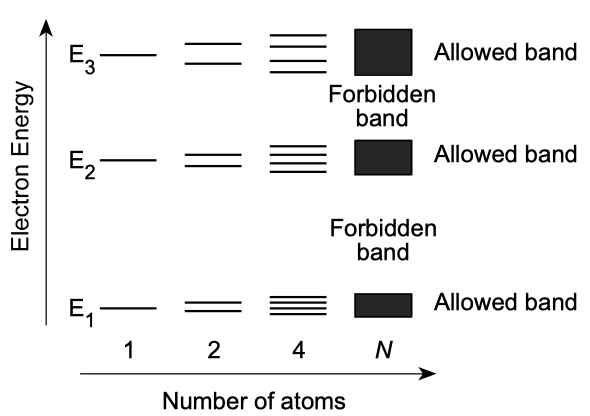
\includegraphics[width=1\linewidth]{image/energybandd.png}
    \end{minipage} 
    \item Forbidden and Allowed bands\\
    Depending on the way in which the electron shells interact, some bands can overlap each other, forming a continuous band of energies without any breaks. \\
    If The energy bands are separated, then we end up with forbidden bands between allowed bands.
    \begin{figure}[h]
        \centering
        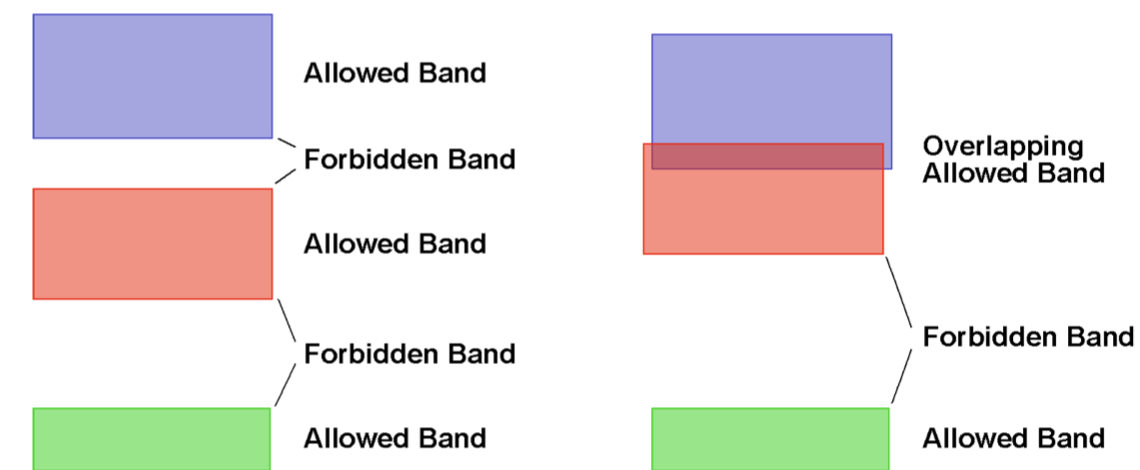
\includegraphics[width=0.75\linewidth]{image/forbidden.png}
    \end{figure}
    When the bands are formed beyond the vacuum level, electrons are free and can take on any energy value.
    \item Electrical Conduction \\
    For the energy to conduct electricity, it has to be a \textbf{Partially-filled Band}. \\
    This allows us to explain the conduction behaviour in solids. Good conductors of electricity because they have partially filled bands.
    \item Insulators \\
    For most ionically and covalently bonded solids, they have filled valance bands. The bandgap between the valance band and conducting band is typically several $eV$.
    \item Semiconductor \\
    Band diagram for semiconductors is basically the same as an insulator. The difference is that the bandgap is much smaller.
    \begin{figure}[h]
        \centering
        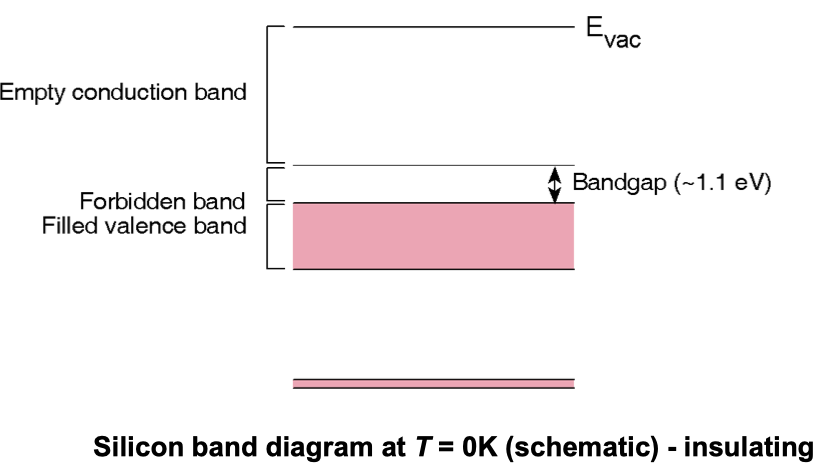
\includegraphics[width=0.75\linewidth]{image/semibandgap.png}
    \end{figure}
    Typical Bandgaps 
    \begin{table}[h!]
      \centering
      \caption{Bandgaps of selected semiconductors at 300K}
      \begin{tabular}{lc}
        \toprule
        Semiconductor & Band gap in eV at 300 K \\
        \midrule
        Silicon (Si) & 1.12 \\
        Germanium (Ge) & 0.66 \\
        Gallium Arsenide (GaAs) & 1.42 \\
        Indium Antimonide (InSb) & 0.17 \\
    
        \midrule
        \multicolumn{2}{l}{Note: Bandgap varies slightly with temperature} \\
        \midrule
        Insulator & Band gap in eV at 300 K \\
        \midrule
        Silicon Dioxide (SiO2) &  $>>$ 9 \\
        Silicon Nitride (Si3N4) &  $>>$ 5 \\
    
        \bottomrule
      \end{tabular}
    \end{table}
    \newpage
    \item Energy Band Diagrams \\
    \begin{figure}[h]
        \centering
        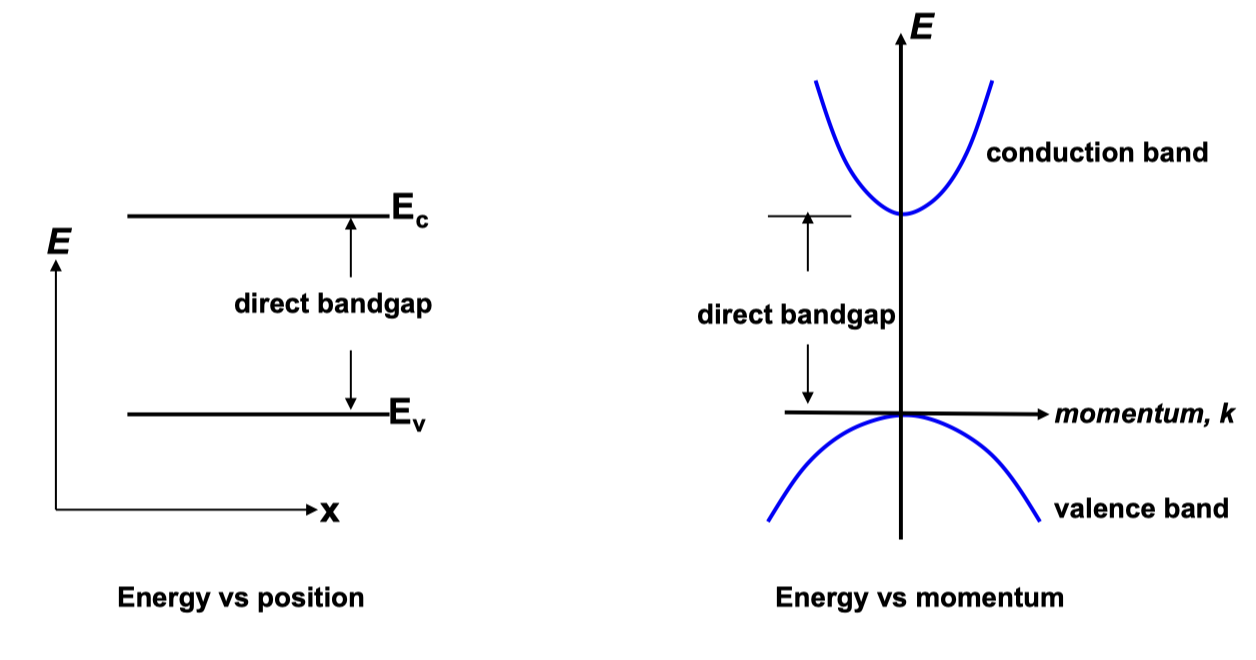
\includegraphics[width=0.75\linewidth]{image/bandgapdiagram.png}
    \end{figure}
    \item Optical Processes in Semiconductors
    \begin{figure}[h]
        \centering
        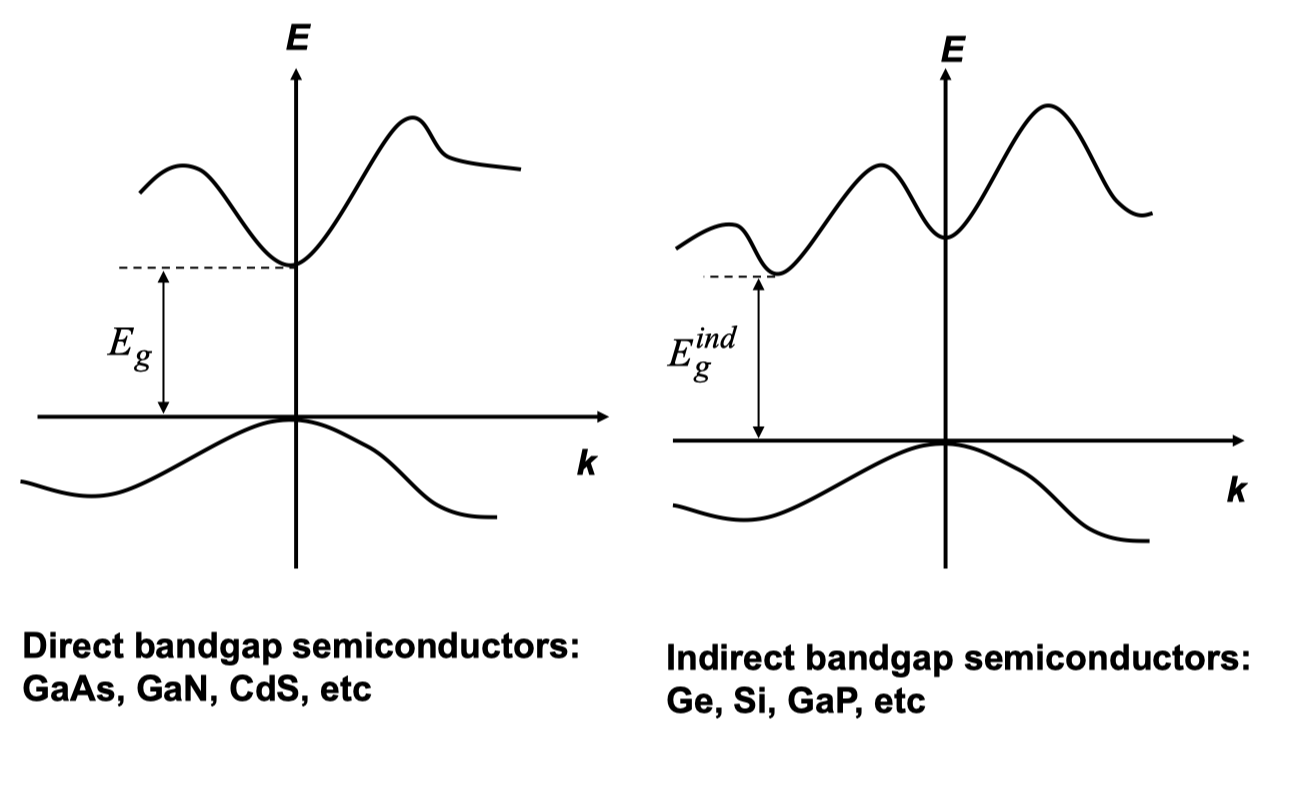
\includegraphics[width=0.75\linewidth]{image/opticalprocesssemincon.png}
    \end{figure}
    \item Direct and indirect band diagram\\
    The luminescence process involve three separae steps
    \begin{enumerate}
        \item Excitation: Electron-hole pair have to be excited by an external source of energy
        \item Thermalization: Excited e-h pairs relax towards quasi-thermal-equilibrium distributions via emitting phonon energy (lattice vibration).
        \item Recombination: The thermalized e-h pairs recombine radiatively to produce the emission of photon energy = $E_g$. Fixed $E_g$ $\rightarrow$ fixed wavelength.
    \end{enumerate}
    \item Absorption of light in a semiconductor \\
    \begin{figure}[h]
        \centering
        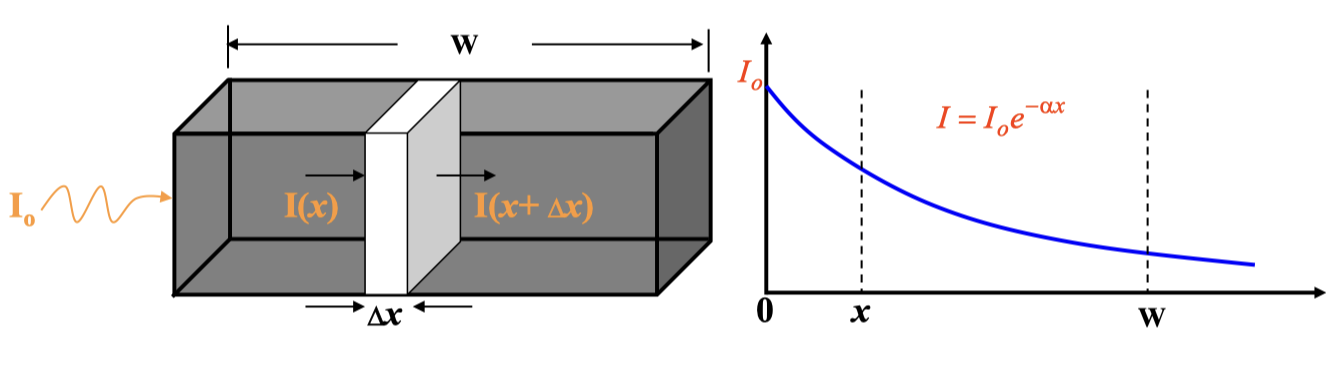
\includegraphics[width=1\linewidth]{image/absorption.png}
    \end{figure}
    \begin{equation}
        I = I_0e^{-\alpha x}
    \end{equation}
    Where $\alpha$ is the absorption coefficient which is ranged from $10^2 - 10^5$\unit{cm^{-1}}.
\end{enumerate}


\newpage